\documentclass[16pts]{report}
\usepackage[utf8]{inputenc}
\usepackage[T1]{fontenc}
\usepackage[francais]{babel}
\usepackage{xcolor}
\usepackage[hyphens]{url}
\usepackage[hidelinks]{hyperref}
\usepackage{amsmath}
\usepackage{graphicx}
\usepackage{geometry}
\usepackage{textcomp}
\usepackage{wrapfig}
\usepackage{lscape}
\usepackage{rotating}
\hypersetup{hypertexnames=true}
\geometry{hmargin=2.5cm,vmargin=1.5cm}

\usepackage{float} %Option H pour les figures, utile.

%\maketitle
%\clearpage

\begin{document}
\bibliographystyle{unsrt}
\nocite{*}

\chapter{Organisation}
\label{cha:Organisation}

\section{Fonctionnement de l'équipe}
\label{sec:Fonctionnement de l'équipe}

Nous avions déjà décidé assez rapidement au début de l'année de Master 
de former notre groupe pour le projet de programmation. Lors du choix 
des sujets, nous avons pris en compte les préférences de chacun et nous 
avons ainsi pu choisir ce sujet. Celui-ci nous a tout de suite intéressés 
puisque c'était avant tout un projet concret qui vise à répondre à un 
réel besoin.
En ce qui concerne la mise en place des bases de notre travail en 
équipe, nous avons réussi à nous organiser rapidement. 
\\
Dès le début, nous avons commencé à répartir nos tâches, ce qui nous a 
permis d’avancer plus rapidement que ce soit dans l’analyse ou, plus tard, 
dans la conception. Il était très important pour nous de bien les séparer, 
car malgré un échange d’informations constant avec des outils tels que 
Git ou Google Drive, il était parfois difficile de travailler à plusieurs 
sur une même tâche sans se gêner mutuellement. Les sessions de travail 
individuelles étaient souvent suivies de réunion, afin de rassembler 
les travaux de chacun.
\\


\section{Gestion du projet}
\label{sec:Gestion du projet}

\begin{enumerate}
	% \item Planning initial du projet
	% \\
	% Ébauche de la bibliographie et de l'existant	==> 06/01 à 17/01
	% Ébauche des besoins et des tests				==> 20/01 à 09/02
	% Ébauche de l'architecture						==> 03/02 à 14/02
	% Codage de l'application	(Show only subtaks)		==> 19/02 à 29/03
	% 	Interface et Fonctionnalités				==> 19/02 à 29/03
	% 	Recherche (Conflits et Matériel)			==> 19/02 à 18/03
	% 	Tests										==> 03/03 à 29/03
	% Réalisation du rapport final					==> 31/03 à 08/04
	% Réalisation des manuels ???						==> 04/04 à 08/04
	% Réalisation du diaporama						==> 08/04 à 14/04


	% \item Planning final du projet
	% \\
	% Ébauche de la bibliographie et de l'existant	==> 06/01 à 24/01
	% Ébauche des besoins et des tests				==> 20/01 à 09/02
	% Ébauche de l'architecture						==> 03/02 à 16/02
	% Codage de l'application	(Show only subtaks)		==> 19/02 à 08/04
	% 	Interface et Fonctionnalités				==> 19/02 à 05/04
	% 	Recherche (Conflits et Matériel)			==> 19/02 à 18/03
	% 	Tests										==> 03/03 à 07/04
	% Réalisation du rapport final					==> 31/03 à 08/04
	% Réalisation des manuels ???						==> 04/04 à 08/04
	% Réalisation du diaporama						==> 08/04 à 14/04
	% \\


	\begin{sidewaysfigure}[ht]
		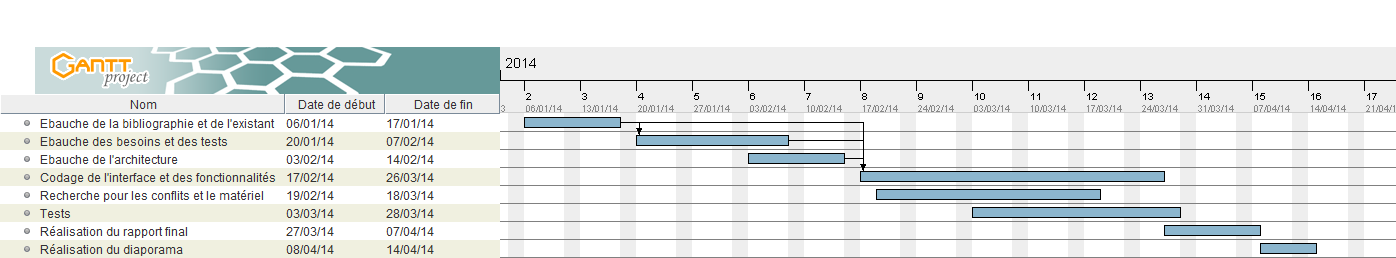
\includegraphics[scale=0.5]{../illustrations/planning_initial_pdp.png}
		\centering
		\caption{Planning initial du projet}
		\label{fig:PlanningInitial}
	\end{sidewaysfigure}

	\begin{sidewaysfigure}[ht]
		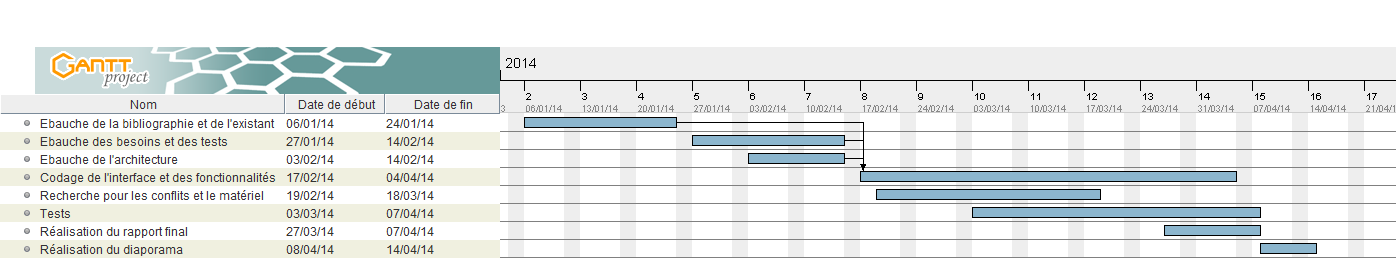
\includegraphics[scale=0.5]{../illustrations/planning_final_pdp.png}
		\centering
		\caption{Planning final du projet}
		\label{fig:PlanningFinal}
	\end{sidewaysfigure}

	\item Commentaires critiques

	Voici le planning prévisionnel de la réalisation de nos tâches durant 
	notre projet ainsi que le planning final. Lors du commencement de notre 
	projet, nous n'avions pas formalisé ce planning avec ce schéma, mais nous 
	avions listé les principales tâches avec le temps que ça allait 
	nous prendre.
	\\
	On peut constater que chaque tâche ne s'est pas déroulée comme prévu, 
	en effet, notre projet a nécessité une grande phase de recherche sur le 
	problème de résolution des conflits et de détection du matériel, la 
	réalisation des différents tests a duré plus longtemps 
	(NOMBRE DE JOURS en plus -- FIXME).
	\\
	Ensuite, durant la phase de conception, nous avons pu modifier 
	certaines tâches. En effet, la résolution des conflits a été écartée pour simplement aider l'utilisateur à trouver les options qui posent	problème et en le laissant corriger le problème seul. L'idée de détecter 
	automatiquement le matériel de l'utilisateur pour lui proposer une 
	configuration a été abandonnée au profit d'un site communautaire 
	contenant des relations entre des options et du matériel.



\end{enumerate}

\section{Logiciels et technologies utilisées}
\label{sec:Logiciels et technologies utilisés}

Git (1.9.0) est un logiciel de gestion de versions décentralisé.
C'est un logiciel libre créé par Linus Torvalds.
Git fonctionne de façon décentralisée, mais nous utilisons les serveurs de 
Github pour gérer notre dépôt.
Nous avons utilisé ce logiciel afin de faciliter le travail collaboratif.
\\
Google drive (1.14) est un service de stockage et de partage de fichiers 
dans le Cloud. Nous l'avons utilisé afin de pouvoir partager des documents 
sans avoir à les mettre sur notre dépôt Git. 
\\
LucidChart est un service qui permet de travailler collaborativement à la 
réalisation de différents diagrammes. Nous nous sommes servis de celui-ci 
afin de réaliser les différents diagrammes relatifs à notre analyse.
\\
Texmaker (4.1.1) est un logiciel libre destiné à l'édition de documents 
LaTeX. Il est possible de visionner le rendu de notre texte directement dans 
celui-ci. Nous l'avons utilisé afin de compiler nos fichiers LaTeX en PDF.
\\
Python (2.7.6) est un langage de programmation objet multiplateformes. 
Il favorise la programmation impérative structurée et orientée objet. Il 
est doté d'un typage dynamique fort, d'une gestion automatique de la 
mémoire par ramasse-miettes. Il est similaire au Perl, Ruby et Smalltalk. 
Nous avons décidé d'utiliser ce langage, dans un premier temps pour 
faciliter l'utilisation d'une bibliothèque python que nous avons trouvé 
mais également pour simplifier la portabilité de l'application finale.
\\
GTK+ (3.8.5) est un ensemble de bibliothèques logicielles, c'est-à-dire 
un ensemble de fonctions permettant de réaliser des interfaces graphiques. 
Nous avons eu le choix entre GTK et QT pour l'interface graphique de notre 
application, et nous avons choisi GTK principalement, car certain 
d'entre nous l'avaient déjà utilisé auparavant. D'un point de vue 
fonctionnel, les deux bibliothèques sont tout aussi performantes dans 
la plupart des cas.
\\
PHP5, MySQL, HTML5, CSS3 et Javascript. Nous avons utilisé ces différents 
langages afin de créer le site de notre projet. Le couple PHP5 et MySQL 
ont permis de faire la liaison entre le site et la base de données. Les 
langages HTML5 et CSS3 permettent de gérer le contenu et son agencement. 
Enfin, le Javascript a permis de gérer les différents évènements sur la 
page à l'aide du Framework JQuery (2.1.0). Nous avons également utilisé 
le Framework Bootstrap (3.1.1) afin d'avoir un design simple et rapide à 
mettre en place pour le site.


\end{document}
